% =====================================================================
% Snippet: stage-container.tex
% =====================================================================
% USAGE: Stage container with title bar + internal content zone.
% This is the BACKBONE for stage-based horizontal layouts like
% test-gat (5 stages: Molecule / GAT Layer / Multi-Head / Prediction
% / Interpret). Each stage is self-contained with its own title,
% color tone, and internal anchor points.
%
% Copy %% COPY-START / END, replace:
%   - stage_id: numeric (s1, s2, ...) for anchor naming
%   - title: stage title (e.g., "Stage 1: Input")
%   - color_line / color_bg: from multi-zone-palette
%   - x, y: top-left anchor
%   - w, h: width, height in cm
%
% Inside the stage: put your snippet content (heatmap / formula / box)
% positioned relative to (s\stage_id.center) or (s\stage_id.north).
% Recommended internal padding: 0.4cm from zone border.
%
% RULE: Multiple stages in a row must have SAME HEIGHT and EQUAL GAP
% between centers (typically 0.5-1.0cm gap).
% =====================================================================

\documentclass[tikz,border=10pt]{standalone}
\usepackage{xcolor,tikz}
\usetikzlibrary{positioning,calc,fit}

\definecolor{acaTealLine}{HTML}{1F8F8F}
\definecolor{acaTealBg}{HTML}{D3EBEB}
\definecolor{acaBlueLine}{HTML}{3060A8}
\definecolor{acaBlueBg}{HTML}{DCE6F4}
\definecolor{acaPurpleLine}{HTML}{6E3FA0}
\definecolor{acaPurpleBg}{HTML}{EDE3F6}
\definecolor{acaOrangeLine}{HTML}{D06020}
\definecolor{acaOrangeBg}{HTML}{F9E0D0}
\definecolor{acaGreenLine}{HTML}{389050}
\definecolor{acaGreenBg}{HTML}{DBEDDC}

\tikzset{
  stage zone/.style={
    rectangle, rounded corners=4pt,
    line width=0.7pt, draw=#1,
    fill=#1!8,           % very light tint (~8% saturation)
    inner sep=0pt,
  },
  stage title/.style={
    rectangle, rounded corners=2pt,
    fill=#1!90, draw=#1, line width=0.5pt,
    text=white, font=\small\bfseries,
    inner sep=4pt, inner ysep=2pt,
  },
}

\begin{document}
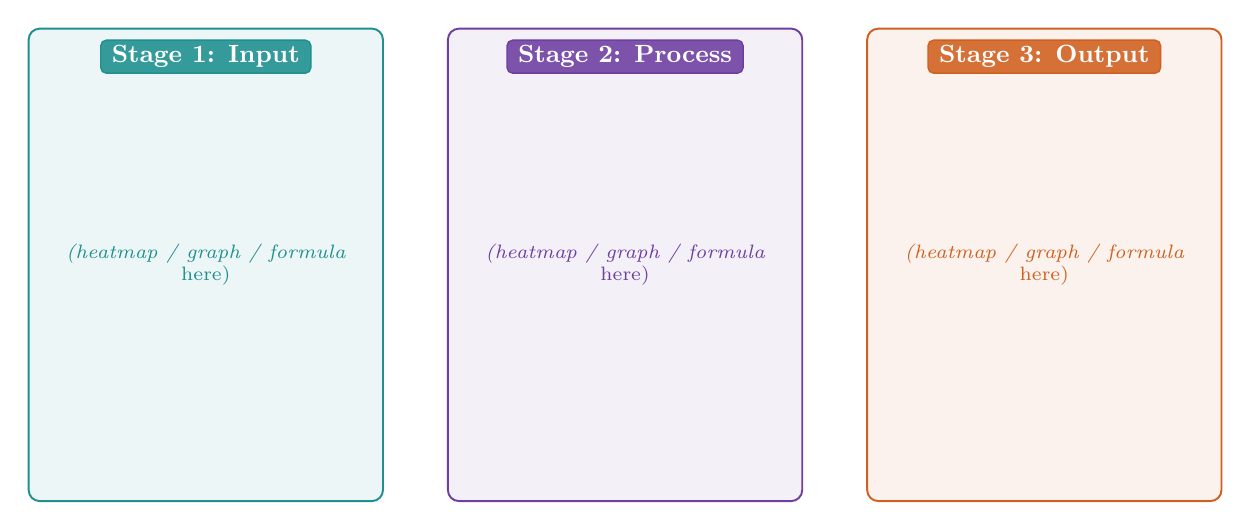
\begin{tikzpicture}

%% COPY-START =========================================================

% --- DEMO: 3 stages side by side ---
% In your figure, change colors / titles / widths to match your domain.
\def\stageW{4.5}    % cm — stage width
\def\stageH{6.0}    % cm — stage height
\def\stageGap{0.8}  % cm — gap between stages

% Stage 1 (Teal)
\node[stage zone=acaTealLine,
      minimum width=\stageW cm, minimum height=\stageH cm,
      anchor=north west]
  (s1) at (0, 0) {};
\node[stage title=acaTealLine, anchor=north]
  at ([yshift=-0.15cm]s1.north) {Stage 1: Input};
% --- INSIDE stage 1: put your snippet content here ---
\node[font=\scriptsize, anchor=center, align=center, color=acaTealLine]
  at (s1.center) {\itshape (heatmap / graph / formula\\here)};

% Stage 2 (Purple)
\node[stage zone=acaPurpleLine,
      minimum width=\stageW cm, minimum height=\stageH cm,
      anchor=north west]
  (s2) at ($(s1.north east) + (\stageGap, 0)$) {};
\node[stage title=acaPurpleLine, anchor=north]
  at ([yshift=-0.15cm]s2.north) {Stage 2: Process};
\node[font=\scriptsize, anchor=center, align=center, color=acaPurpleLine]
  at (s2.center) {\itshape (heatmap / graph / formula\\here)};

% Stage 3 (Orange)
\node[stage zone=acaOrangeLine,
      minimum width=\stageW cm, minimum height=\stageH cm,
      anchor=north west]
  (s3) at ($(s2.north east) + (\stageGap, 0)$) {};
\node[stage title=acaOrangeLine, anchor=north]
  at ([yshift=-0.15cm]s3.north) {Stage 3: Output};
\node[font=\scriptsize, anchor=center, align=center, color=acaOrangeLine]
  at (s3.center) {\itshape (heatmap / graph / formula\\here)};

%% COPY-END ===========================================================

\end{tikzpicture}
\end{document}
